%Om filen typsätts som del av hela rapporten så finns \master definierat i början och ingen \begin{document} och \end{document} får finnas, men för att kunna typsätta filen för sig är dem ett måste! \newcommand{\master}{} krävs i början på huvudrapporten!
\ifdefined\master
\else
	\documentclass[twocolumn]{article}
	\usepackage{graphicx}
	\usepackage{float}
	%\input{preamble}
	\begin{document}
\fi
\subsection{Exports}
The program has four different choices for exporting the obtained data; copy to clipboard, save as image, create LaTeX report and create Microsoft Word report.  (Fig. \ref{fig:funcgen})

\subsubsection*{Clipboard}
Copies the figure to clipboard. Textboxes enable the user to modify title and axis labels before copying. (Fig. \ref{fig:funcgen})

\begin{figure}[H]
\centering
\fbox{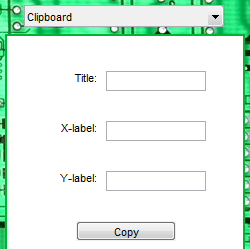
\includegraphics[width=4cm]{Figure/clipboard.png}}
\caption{Copy to clipboard export settings.}
\label{fig:clip}
\end{figure}

\subsubsection*{Image}
Saves the image to disk. Textboxes enable the user to modify title and axis labels before copying. (Fig. \ref{fig:img})

\begin{figure}[H]
\centering
\fbox{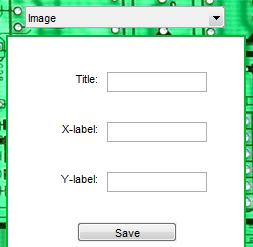
\includegraphics[width=4cm]{Figure/image.png}}
\caption{Image export settings.}
\label{fig:img}
\end{figure}

\subsubsection*{LaTeX}
Generates LaTeX report containing the figure. \emph{Image name} textbox enables user to choose file name and format for the figure, which will be saved at the same location as the tex-file. \emph{Caption}, \emph{label} and \emph{width} properties are transferred to corresponding LaTeX commands, while tite and labels are applied directly to the figure before exporting. (Fig. \ref{fig:funcgen})

\begin{figure}[H]
\centering
\fbox{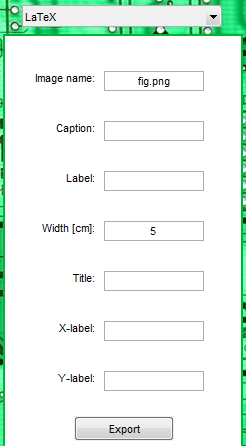
\includegraphics[width=4cm]{Figure/latex.png}}
\caption{LaTeX export settings.}
\label{fig:tex}
\end{figure}

\subsubsection*{Word}
Generates Microsoft Word report containing the figure. \emph{Title}, \emph{x-label} and \emph{y-label} overrides the settings of the figure and the caption is inserted on a centred line below. (Fig. \ref{fig:funcgen})

\begin{figure}[H]
\centering
\fbox{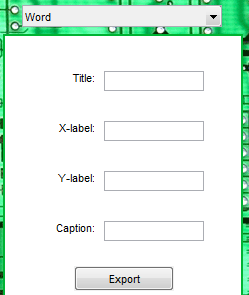
\includegraphics[width=6cm]{Figure/word.png}}
\caption{Word export settings.}
\label{fig:word}
\end{figure}

\ifdefined\master
\else
	\end{document}
\fi